\documentclass[11pt]{article}

% Packages
\usepackage{hyperref} 
\usepackage{amssymb}
\usepackage{amsthm}
\usepackage{amsfonts}
\usepackage{amsmath}
\usepackage{xcolor,bbold}
\usepackage{enumitem}
\usepackage{graphicx}
\usepackage{geometry}
\usepackage{fancyhdr}
\usepackage{setspace}
\usepackage{bm}

\usepackage[
backend=biber, 
citestyle=ieee,
sorting=nyt,    
doi=false,
url=false,
isbn=false,
giveninits=true,
maxbibnames=9999,
hyperref]{biblatex}

\addbibresource{HSI.bib} 

% Page style
\geometry{top=1in,bottom=1in,left=1in,right=1in}
\setlength{\headheight}{13.6pt}
\pagestyle{fancy}
\doublespacing

% Document settings
\textheight=8.5truein
\textwidth=6.0truein

% Header information
\lhead{Juntang Wang}
\rhead{Fall 2024}
\chead{Minutes}

\begin{document}

\section{Results}
% Juntang 09/29/2024

\begin{figure}[htbp]
    \centering
    % Indian Pines and KSC Figures
    \begin{minipage}{0.45\textwidth}
        \centering
        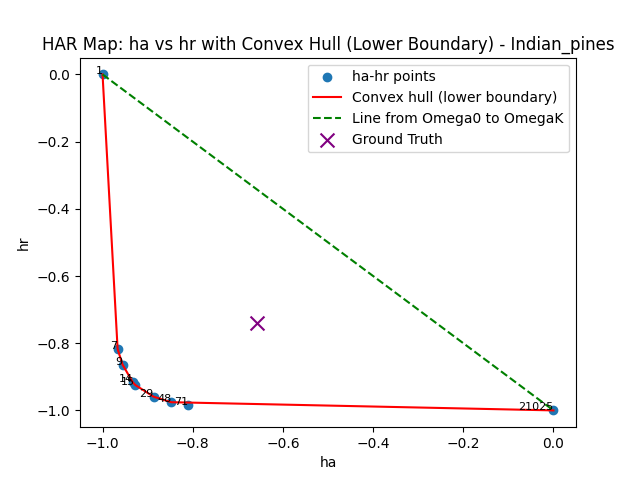
\includegraphics[width=\linewidth]{figures/Indian_pines_HARmap.png}
        \caption{Indian Pines HARmap}
        \label{fig:indian_pines_har}
    \end{minipage}\hfill
    \begin{minipage}{0.45\textwidth}
        \centering
        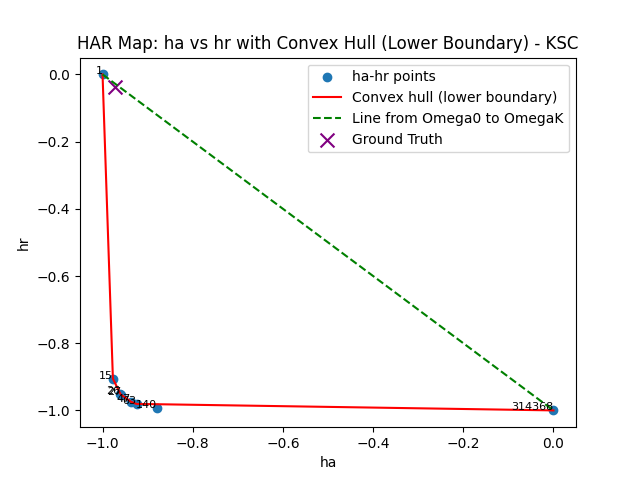
\includegraphics[width=\linewidth]{figures/KSC_HARmap.png}
        \caption{KSC HARmap}
        \label{fig:ksc_har}
    \end{minipage}
\end{figure}

\begin{figure}[htbp]
    \centering
    % Salinas and Salinas-A Figures
    \begin{minipage}{0.45\textwidth}
        \centering
        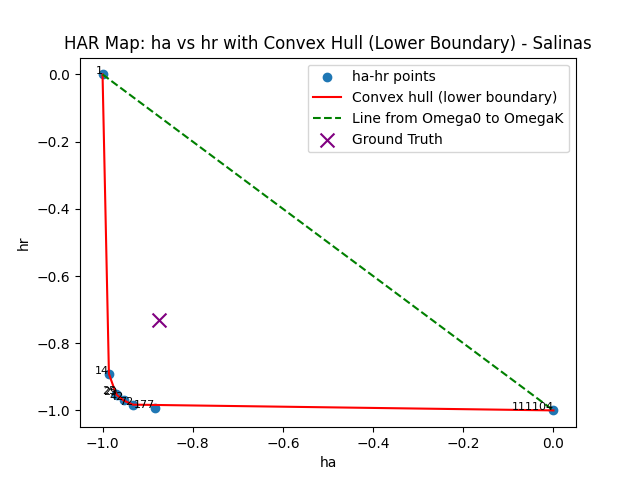
\includegraphics[width=\linewidth]{figures/Salinas_HARmap.png}
        \caption{Salinas HARmap}
        \label{fig:salinas_har}
    \end{minipage}\hfill
    \begin{minipage}{0.45\textwidth}
        \centering
        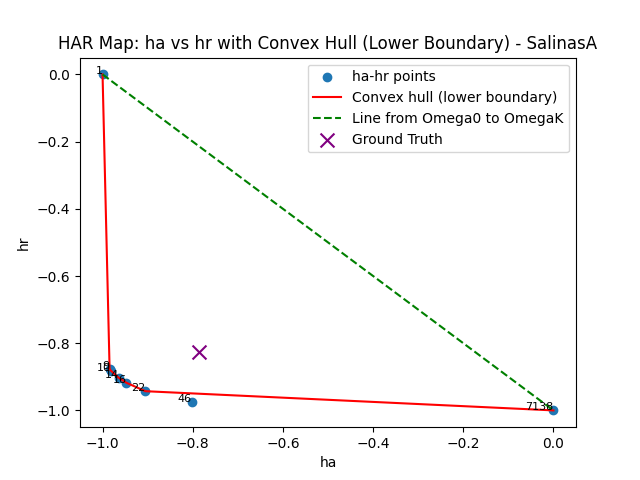
\includegraphics[width=\linewidth]{figures/SalinasA_HARmap.png}
        \caption{Salinas-A HARmap}
        \label{fig:salinasa_har}
    \end{minipage}
\end{figure}

The Hamiltonian functions used in this method are defined as follows:

\[
h_a = - \sum_{C \in \Omega} \alpha(C, C)
\]
\[
h_r = \sum_{C \in \Omega} \alpha^2(C, V)
\]


\begin{figure}[htbp]
    \centering
    % Pavia University Figure
    \begin{minipage}{0.45\textwidth}
        \centering
        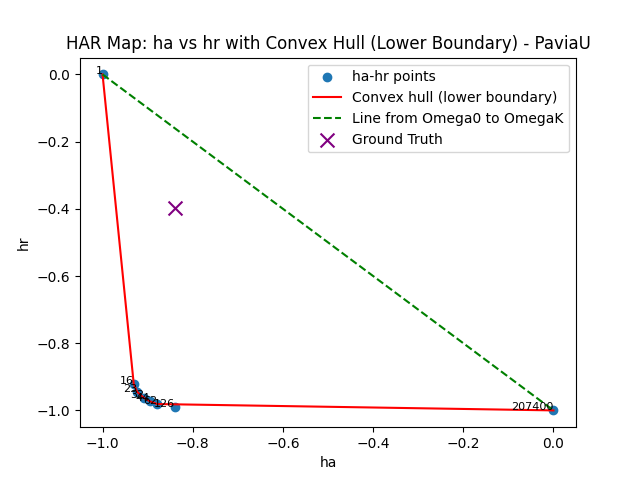
\includegraphics[width=\linewidth]{figures/PaviaU_HARmap.png}
        \caption{Pavia University HARmap}
        \label{fig:pavia_university_har}
    \end{minipage}\hfill
    \begin{minipage}{0.45\textwidth}
    \end{minipage}
\end{figure}

\newpage
\begin{figure}[htbp]
    \centering
    % WHU-Hi Figures
    \begin{minipage}{0.45\textwidth}
        \centering
        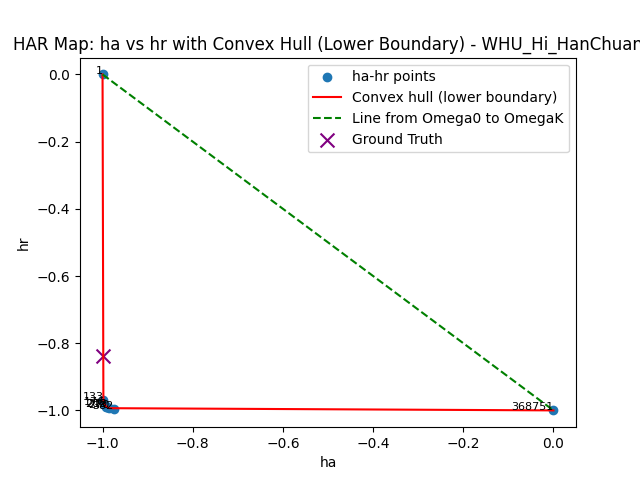
\includegraphics[width=\linewidth]{figures/WHU_Hi_HanChuan_HARmap.png}
        \caption{WHU Hi HanChuan HARmap}
        \label{fig:whu_hanchuan_har}
    \end{minipage}\hfill
    \begin{minipage}{0.45\textwidth}
        \centering
        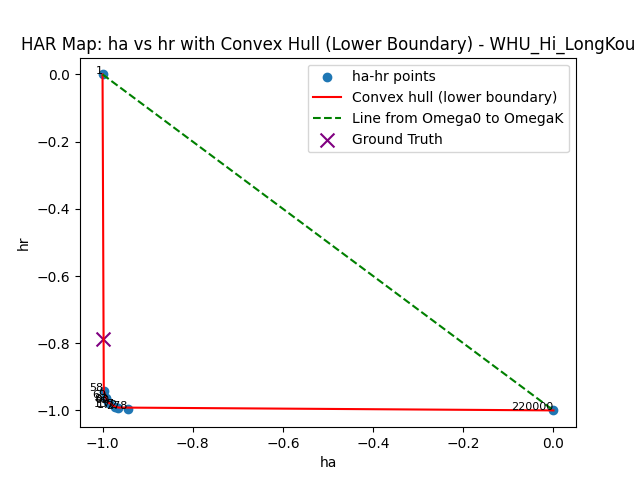
\includegraphics[width=\linewidth]{figures/WHU_Hi_LongKou_HARmap.png}
        \caption{WHU Hi LongKou HARmap}
        \label{fig:whu_longkou_har}
    \end{minipage}
\end{figure}

\section{Datasets}
% Juntang, 09/29/2024
    
    \begin{table}[h!]
    \centering
    \caption{Summary of hyperspectral datasets}
    \label{tab:datasets}
    \resizebox{0.8\textwidth}{!}{
    \begin{tabular}{lccccccl}
    \hline
    \textbf{Dataset} & \textbf{\#x} & \textbf{\#y} & \textbf{\#\bm{$\lambda$}} & \textbf{\bm{$\lambda$} (nm)} & \textbf{\#C} & \textbf{Res. (m)} & \textbf{Year}\\
    \hline
    Indian Pines & 145 & 145 & 220 & 400--2500 & 16 & 20 & 1992\\
    KSC& 512& 614& 176& 400--2500 & 13& 18&1996\\
    Salinas & 512 & 217 & 204 & 400--2500 & 16 & 3.7 & 1998\\
    Salinas-A & 86 & 83 & 204 & 400--2500 & 6 & 3.7 & 1998\\
    Botswana& 1476& 256& 145& 400--2500& 14& 30&2001\\
    Pavia & 1096 & 1096 & 102 & 430--860~ & 9 & 1.3 & 2003\\
    Pavia University & 610 & 610 & 103 & 430--860~ & 9 & 1.3 & 2003\\
    WHU-Hi-HanChuan & 1217 & 303 & 274* & 400--1000& 16 & 0.109 & 2016\\
    WHU-Hi-HongHu & 940 & 475 & 270* & 400--1000& 22 & 0.043 & 2017\\
    WHU-Hi-LongKou & 550 & 400 & 270* & 400--1000& 9 & 0.463 & 2018\\
    BigEarthNet-S2-s & 1200& 1200& 13& 443--2190& 12& 10-60& 2017\\
    \hline
    \end{tabular}
    }
    \end{table}



    
    \begin{figure}[htbp]
        \centering
        \includegraphics[width=0.5\linewidth]{output1.png}
        \caption{Teasors' Plot}
        \label{fig:tp}
    \end{figure}
    \newpage

Indian Pines: \cite{baumgardner220BandAVIRIS}, KSC, Salinas, Salinas-A, Botswana, Pavia and Pavia University: \cite{ehu_datasets}, WHU-Hi-HanChuan, WHU-Hi-HongHu, WHU-Hi-LongKou: \cite{zhongMiniUAVborneHyperspectralRemote2018, huWHUhiUAVborneHyperspectral}, BigEarthNet-S2-s: \cite{clasen2024refinedbigearthnet, hackel2024configilm}.

\printbibliography

\end{document} 
